\chapter{Introduction}
\label{chap:introduction}

\section{Spacecraft fire safety}

Fire safety is a system-level requirement for crewed spacecraft. A pressurised
vehicle necessarily contains an oxidising atmosphere, combustible materials,
electrical equipment, and potential ignition sources inside a confined volume.
Unlike a terrestrial building, a spacecraft may not allow rapid evacuation,
replacement of damaged hardware, atmospheric clean-up, or external emergency
support. Fire safety must therefore be considered alongside mass, function,
manufacturability, reliability, and mission architecture rather than treated as
a single material property \cite{guibaud2022spacecraft}.

Apollo~1 remains a defining example of this coupled hazard. During a ground
test on 27 January 1967, a fire developed rapidly in the command module's
high-pressure pure-oxygen atmosphere. The exact ignition source was not
established, although electrical wiring was considered a likely source. The
combination of combustible materials, the oxygen-rich atmosphere, and the
inward-opening hatch made the event catastrophic. The post-fire images in
\cref{fig:apollo1} show why specimen-level flammability cannot be separated
completely from vehicle installation, atmosphere, wiring, and system design.
The accident led to major changes in materials, wiring, hatch design,
atmosphere selection, and test procedures \cite{guibaud2022spacecraft}.

\begin{figure}[htbp]
\centering
\begin{subfigure}[t]{0.48\textwidth}
\centering
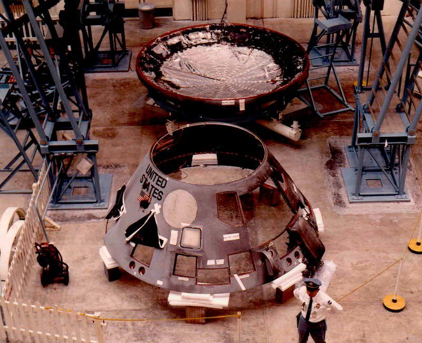
\includegraphics[width=\linewidth,height=0.35\textheight,keepaspectratio]{Apollo1_1.png}
\caption{Apollo 204 command module during the post-fire investigation.}
\end{subfigure}\hfill
\begin{subfigure}[t]{0.48\textwidth}
\centering
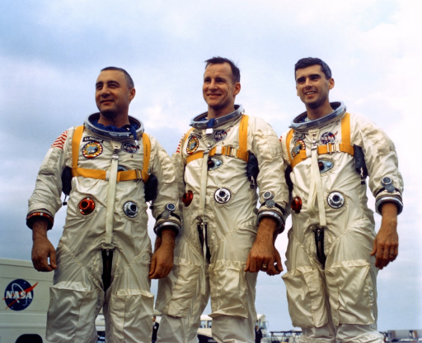
\includegraphics[width=\linewidth,height=0.35\textheight,keepaspectratio]{Apollo1_2.png}
\caption{Prime crew: Grissom, White, and Chaffee.}
\end{subfigure}
\caption{Apollo~1 command module and crew. NASA public-domain photographs
\cite{nasaApolloModule,nasaApolloCrew}.}
\label{fig:apollo1}
\end{figure}

Future exploration increases the consequences of a fire event. Long-duration
missions, lunar or Martian surface operations, and distant spacecraft cannot
assume immediate resupply or rapid return to Earth. At the same time, mission
atmospheres may differ from terrestrial conditions in oxygen concentration,
pressure, gravity, ventilation, and material aging. A material or configuration
qualified in one environment cannot automatically be assumed to retain the same
flammability behaviour in another.

\section{Flammability and flame spread}
\label{sec:intro-flammability}

Flammability is not one quantity. It includes whether a material ignites, how
a flame develops after ignition, how rapidly it spreads, and what combustion
products are produced. The literature database assembled for this work records
five experimental outputs.

\begin{table}[htbp]
\centering
\caption{Five variables used to describe material flammability in the database.}
\label{tab:flammability-variables}
\begin{tabularx}{\textwidth}{@{}p{0.19\textwidth}X@{}}
\toprule
Variable & Engineering interpretation \\
\midrule
Ignition & Whether the imposed energy and environment establish a flame. \\
Flame length & Spatial extent of the visible flame under the test condition. \\
Flame-spread rate (FSR) & Speed of the advancing flame front,
reported in \si{\metre\per\second}. \\
Heat-release rate (HRR) & Rate of chemical energy release,
reported in \si{\watt} when available. \\
Smoke/aerosols & Production of particulate and condensable combustion
products relevant to visibility, toxicity, and detection. \\
\bottomrule
\end{tabularx}
\end{table}

These outputs represent different stages and consequences of a fire. Ignition
describes initiation. Flame length, FSR, and HRR describe flame growth and
severity. Smoke and aerosols affect detection, visibility, toxicity, and
habitability. Their availability is uneven in the published literature.
Consequently, this work develops two supervised-learning tasks for which the
database provides sufficient observations: binary ignition classification and
continuous FSR regression. Flame length, HRR, and smoke/aerosols remain
important database outputs, but they are not used as model predictors because
they are post-outcome quantities.

An established flame can fail at both low and high flow. At high imposed flow
or stretch, the residence time in the reaction zone can become too short for
sustained combustion. This high-flow extinction mechanism is commonly described
as \emph{blowoff}. At very low flow, convective heat feedback and oxygen
transport may be insufficient to offset conductive and radiative losses. The
flame then shrinks and extinguishes through \emph{quenching}.

The low-flow quenching branch is especially relevant in microgravity because
buoyancy no longer imposes a substantial natural-convection velocity. In normal
gravity, buoyant flow can mask this near-zero-flow behaviour. The resulting
relationship between limiting oxygen concentration and imposed flow can be
U-shaped, as illustrated in \cref{fig:flammability-map}. A material may fail
to sustain a flame at both very low and very high flow while remaining
flammable at intermediate flow. Oxygen concentration alone is therefore not a
sufficient descriptor of spacecraft fire risk.

\begin{figure}[htbp]
\centering

\includegraphics[width=0.7\textwidth]{flammability_map.png}
\caption{Schematic U-shaped flammability boundary. The low-velocity branch is
quenching and the high-velocity branch is blowoff; curves show the reported
fuel-width dependence. Reproduced from Johnston et al.\
\cite{johnston2015blowoff}.}
\label{fig:flammability-map}
\end{figure}

The literature review that follows examines spacecraft fire safety, microgravity
combustion, flame-spread modelling, and machine-learning approaches for
heterogeneous experimental databases. It then identifies the research gap,
states the research question and objectives, and motivates the source-aware
evaluation framework developed in the subsequent methodology chapter.